\subsection{File Integrity Module}
File Integrity Monitoring (FIM) is a security process used to monitor the integrity of system and application files. FIM is an important security defense layer for any organization monitoring sensitive assets. It provides protection for sensitive data, application, and device files by monitoring, routinely scanning, and verifying their integrity. It helps organizations detect changes to critical files on their systems which reduces the risk of data being stolen or compromised. This process can save time and money in lost productivity, lost revenue, reputation damage, and legal and regulatory compliance penalties.

Wazuh has a built-in capability for file integrity monitoring. The Wazuh FIM module monitors files and directories and triggers an alert when a user or process creates, modifies, and deletes monitored files. It runs a baseline scan, storing the cryptographic checksum and other attributes of the monitored files. When a user or process changes a file, the module compares its checksum and attributes to the baseline. It triggers an alert if it finds a mismatch. The FIM module performs real-time and scheduled scans depending on the FIM configuration for agents and manager.

\subsubsection{How it works}
The FIM module runs periodic scans on specific paths and monitors specific directories for changes in real time. You can set which paths to monitor in the configuration of the Wazuh agents and manager.

FIM stores the files checksums and other attributes in a local FIM database. Upon a scan, the Wazuh agent reports any changes the FIM module finds in the monitored paths to the Wazuh server. The FIM module looks for file modifications by comparing the checksums of a file to its stored checksums and attribute values. It generates an alert if it finds discrepancies.

The Wazuh FIM module uses two databases to collect FIM event data, such as file creation, modification, and deletion data. One is a local SQLite-based database on the monitored endpoint that stores the data in:
\begin{itemize}
    \item \texttt{C:\textbackslash Program Files (x86)\textbackslash ossec-agent\textbackslash queue\textbackslash fim\textbackslash db} on Windows.
    \item \texttt{/var/ossec/queue/fim/db} on Linux.
    \item \texttt{/Library/Ossec/queue/fim/db} on macOS.
\end{itemize}

The other is an agent database on the Wazuh server. The wazuh-db. daemon creates and manages a database for each agent on the Wazuh server. It uses the ID of the agent to identify the database. This service stores the databases at \texttt{/var/ossec/queue/db}.

\begin{figure} [H]
    \centering
    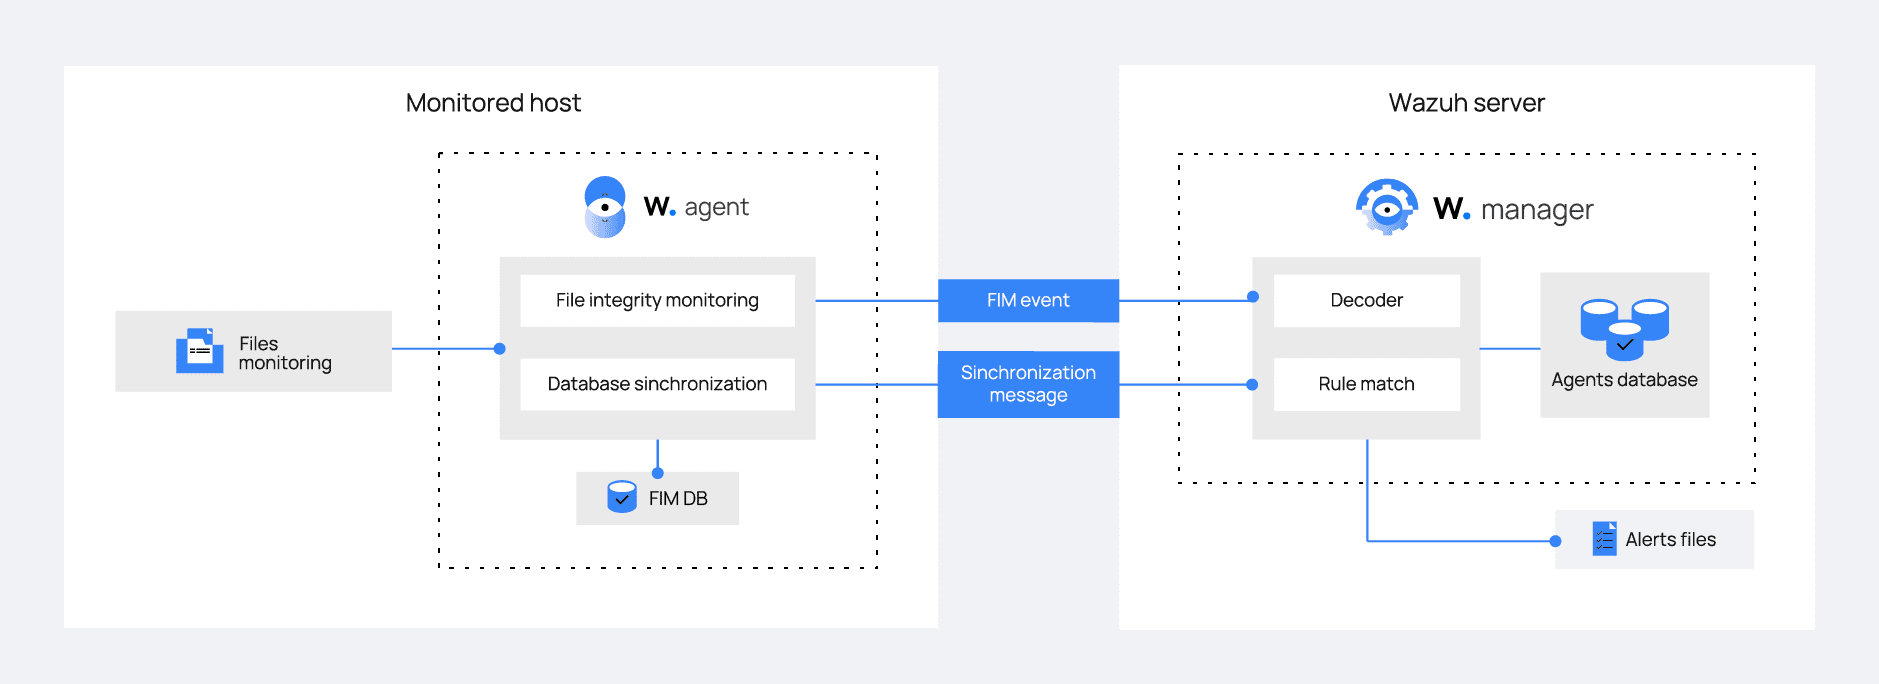
\includegraphics[width=\textwidth]{images/fim/fim-flow.png}
    \caption{Working Flow of Wazuh File Integrity Module}
    \label{fig:fim-flow}
\end{figure}

The FIM module keeps the Wazuh agent and the Wazuh server databases synchronized with each other. It always updates the file inventory in the Wazuh server with the data available to the Wazuh agent. An up-to-date Wazuh server database allows for servicing FIM-related API queries. The synchronization mechanism only updates the Wazuh server with information from the Wazuh agents such as checksums and file attributes that have changed.

The Wazuh agent and manager have the FIM module enabled and pre-configured by default. However, we recommend that you review the configuration of your endpoints to ensure that you tailor the FIM settings, such as monitored paths, to your environment.

\subsubsection{Configuration}
The FIM module runs scans on Windows, Linux, and macOS operating systems. There are both global settings and settings that are specific to the operating system of the endpoint. We discuss these settings and the supported operating systems in the Basic settings section of this guide.

You must specify the directories where the FIM module must monitor the creation, modification, and deletion of files or configure the specific files you need to monitor. You can specify the file or directory to monitor on the Wazuh server and the Wazuh agent configuration files. You can also configure this capability remotely using the centralized configuration file.

You have to set the files and directories to monitor with the directories options. You can include multiple files and directories using comma-separated entries or adding entries on multiple lines. You can configure FIM directories using \texttt{*} and \texttt{?} wildcards in the same way you would use them in a shell or Command Prompt (cmd) terminal. For example, \texttt{C:\textbackslash Users\textbackslash *\textbackslash Downloads}.

Any time the FIM module runs a scan, it triggers alerts if it finds modified files and depending on the changed file attributes. You can view these alerts in the Wazuh dashboard.

Following, you can see how to configure the FIM module to monitor a file and directory. Replace \texttt{FILEPATH/OF/MONITORED/FILE} and \texttt{FILEPATH/OF/MONITORED/DIRECTORY} with your own filepaths.

\begin{itemize}
    \item Add the following settings to the Wazuh agent configuration file, replacing the directories values with your own filepaths:
          \begin{itemize}
              \item Linux: \texttt{/var/ossec/etc/ossec.conf}
              \item Windows: \texttt{C:\textbackslash Program Files (x86)\textbackslash ossec-agent\textbackslash ossec.conf}
              \item macOS: \texttt{/Library/Ossec/etc/ossec.conf}
          \end{itemize}
          \begin{minted}{xml}
<syscheck>
   <directories>FILEPATH/OF/MONITORED/FILE</directories>
   <directories>FILEPATH/OF/MONITORED/DIRECTORY</directories>
</syscheck>
        \end{minted}


    \item Restart the Wazuh agent with administrator privilege to apply any configuration change:
          \begin{itemize}
              \item Linux: systemctl restart wazuh-agent
              \item Windows: Restart-Service -Name wazuh
              \item macOS: /Library/Ossec/bin/wazuh-control restart
          \end{itemize}
\end{itemize}

\subsubsection{Simulation}
We demonstrate the following two use-cases of file integrity module.
\paragraph{Detecting Account Manipulation}
Account manipulation refers to the creation, modification, or deletion of user accounts or other credentials within an organization's IT infrastructure. Monitoring this activity is critical to the cybersecurity of an organization. Unauthorized account manipulations might grant an attacker access to sensitive systems and data.

To maintain persistence on a victim endpoint, adversaries can alter the SSH \texttt{authorized\_keys} file to add their public key. This allows them to access the system remotely without needing to authenticate with a password. We simulate this activity by adding a new public key to the \texttt{authorized\_keys} file.

\subparagraph{Ubuntu endpoint}
\begin{itemize}
    \item We edited the \texttt{/var/ossec/etc/ossec.conf} configuration file and add \texttt{authorized\_keys} for monitoring:
    \begin{minted}{xml}
<syscheck>
    <directories whodata="yes" realtime="yes">/home/*/.ssh/authorized_keys</directories>
</syscheck>
    \end{minted}

    \item  We restarted the Wazuh agent to apply the configuration:
          \begin{minted}{bash}
systemctl restart wazuh-agent
            \end{minted}
    \item We generated an SSH key\-pair for user authentication and saved it as \texttt{.ssh/test\_key} using the following command:
          \begin{minted}{bash}
ssh-keygen -f .ssh/test_key
            \end{minted}
    \item We ran the following command to copy the content of the generated SSH public key \texttt{test\_key.pub} and added it to the \texttt{authorized\_keys} file in the target Ubuntu user \texttt{.ssh} directory.
          \begin{minted}{bash}
cat ~/.ssh/test_key.pub | ssh -i github/cse406/wazuh/wazuh-agent-linux-1_key.pem asifazad@20.205.141.120 "sudo tee -a /home/asifazad/.ssh/authorized_keys"
            \end{minted}
          \begin{figure} [H]
              \centering
              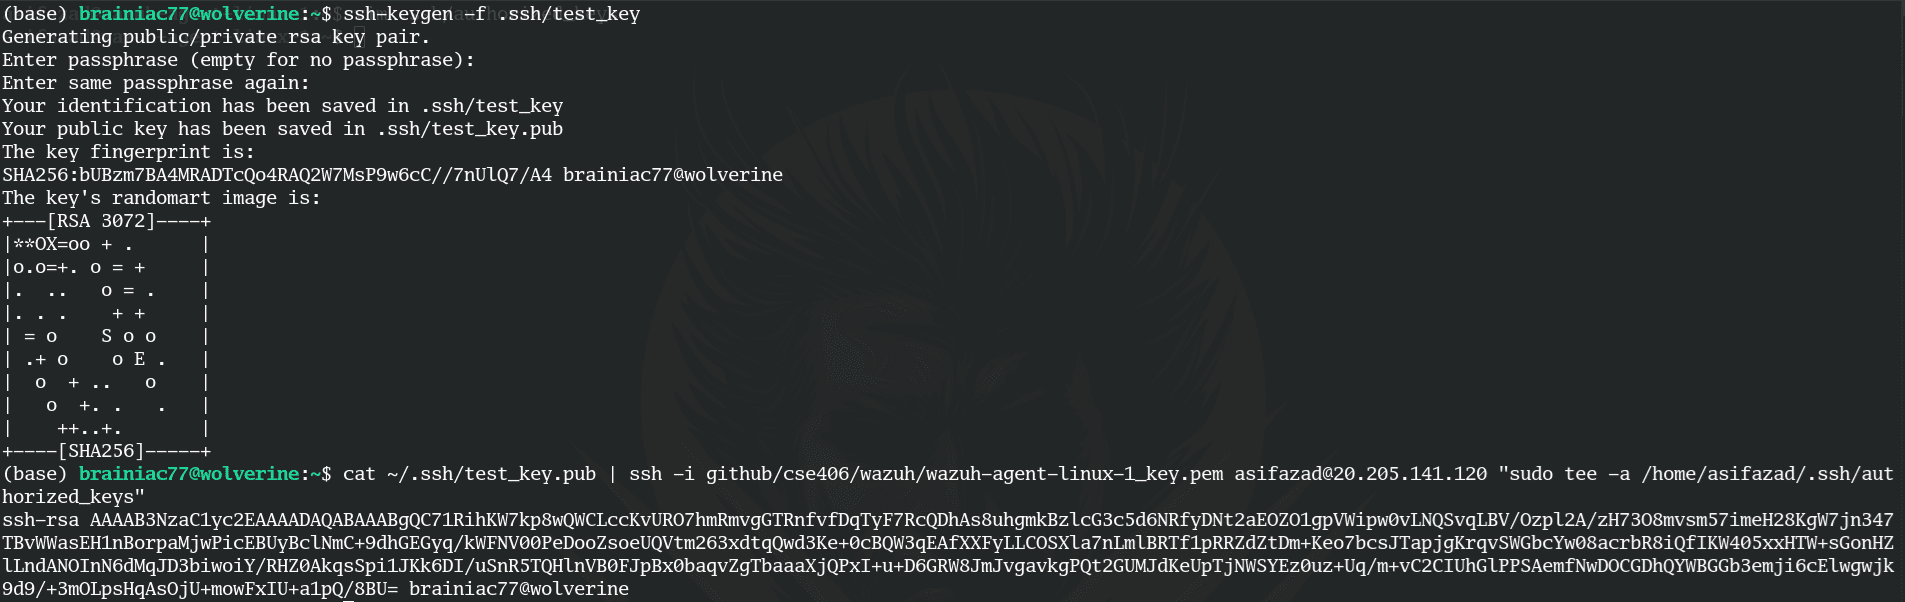
\includegraphics[width=\textwidth]{images/fim/fim-2.png}
              \caption{Testing Commands in Terminal}
              \label{fig:fim-2}
          \end{figure}

\end{itemize}


\paragraph{Monitoring Configuration Changes}
Monitoring configuration changes helps to establish accountability for changes made to systems and applications. Organizations can identify responsible parties and ensure that changes are properly authorized and documented by maintaining a record of changes and who made them.

We can configure the FIM module to monitor configuration files and report any changes. The Wazuh FIM module uses the \texttt{whodata} and \texttt{report\_changes} attributes to record the following information about such changes:

\begin{itemize}
    \item The login user that made the changes.
    \item The time of the changes.
    \item The process that the user executed.
    \item The changes made to the file.
\end{itemize}


\subparagraph{Ubuntu endpoint}
\begin{itemize}
    \item We created a file \texttt{app.conf} in the \texttt{/etc} directory.
    \begin{minted}{bash}
touch /etc/app.conf
    \end{minted}
    \item We edited the \texttt{/var/ossec/etc/ossec.conf} configuration file and add the configuration below:
    \begin{minted}{xml}
<syscheck>
    <directories realtime="yes" check_all="yes" report_changes="yes" whodata="yes">/etc/app.conf</directories>
</syscheck>
    \end{minted}

    \item We restarted the Wazuh agent to apply the configuration changes:
          \begin{minted}{bash}
systemctl wazuh-agent restart
    \end{minted}
    \item We modified the \texttt{/etc/app.conf} file by using vim with root privilege:
          \begin{minted}{bash}
vim /etc/app.conf
    \end{minted}
    \item We added \texttt{updated image to V2} to the file and save.
\end{itemize}

\subsubsection{Dashboard Update}
\paragraph{Detecting Account Manipulation}
\begin{itemize}
    \item We navigated to \texttt{Modules > Integrity monitoring} on the Wazuh dashboard to view the alert generated when the FIM module detects changes to the \texttt{authorized\_keys} file.
          \begin{figure} [H]
              \centering
              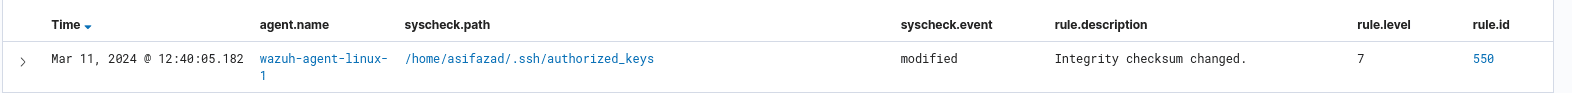
\includegraphics[width=\textwidth]{images/fim/fim-11.png}
              \caption{Alert for Change in \texttt{authorized\_keys} File}
              \label{fig:fim-11}
          \end{figure}
    \item We extended the alert for detailed information.
          \begin{figure} [H]
              \centering
              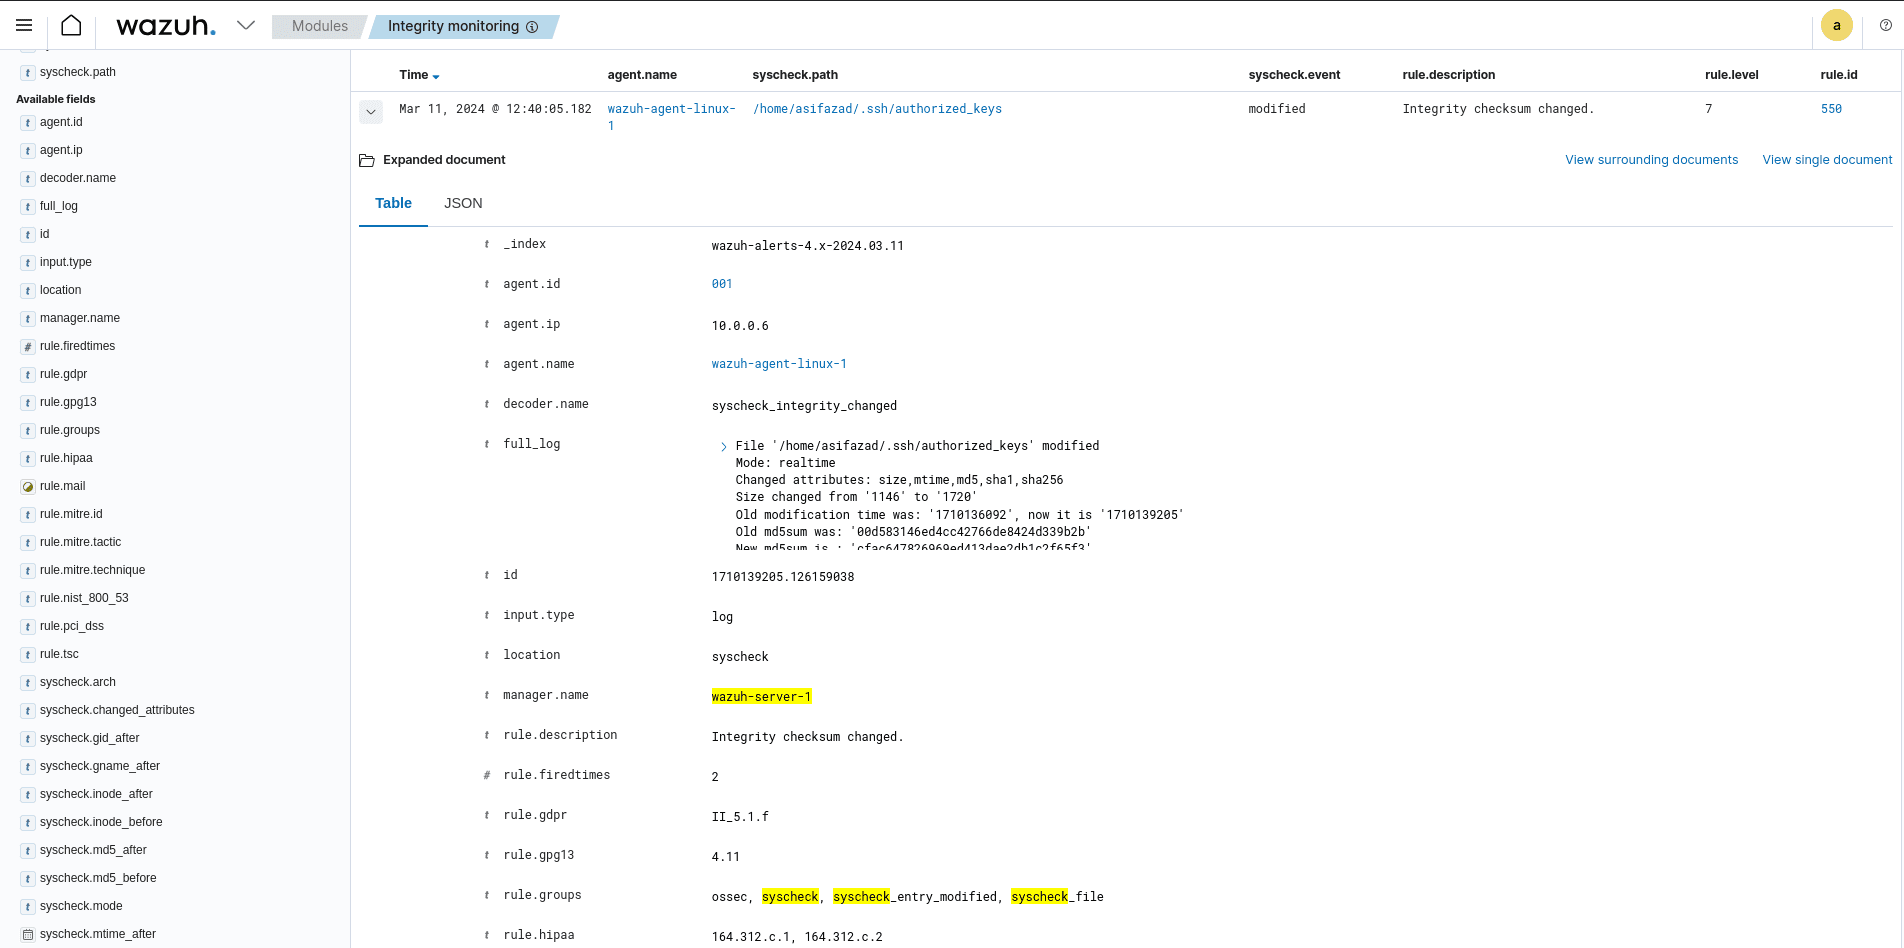
\includegraphics[width=0.75\textwidth]{images/fim/fim-12.png}
              \caption{Alert Details for Change in \texttt{authorized\_keys} File}
              \label{fig:fim-12}
          \end{figure}

\end{itemize}

\paragraph{Monitoring Configuration Changes}
\begin{itemize}
    \item We navigated to \texttt{Modules > Integrity} monitoring on the Wazuh dashboard to view the alert generated when the FIM module detects modification of the configuration file.
          \begin{figure} [H]
              \centering
              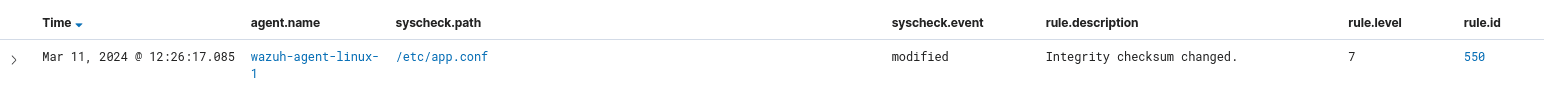
\includegraphics[width=\textwidth]{images/fim/fim-6.png}
              \caption{Alert for Change in \texttt{/etc/app.conf} File}
              \label{fig:fim-6}
          \end{figure}

    \item We expanded the alert to get more information about the event. In this example, the vim text editor modified the configuration file. The logged-in user on the endpoint was ubuntu. The user modified the file using root privilege. The content added to the file is \texttt{updated image to V2}.
          \begin{figure} [H]
              \centering
              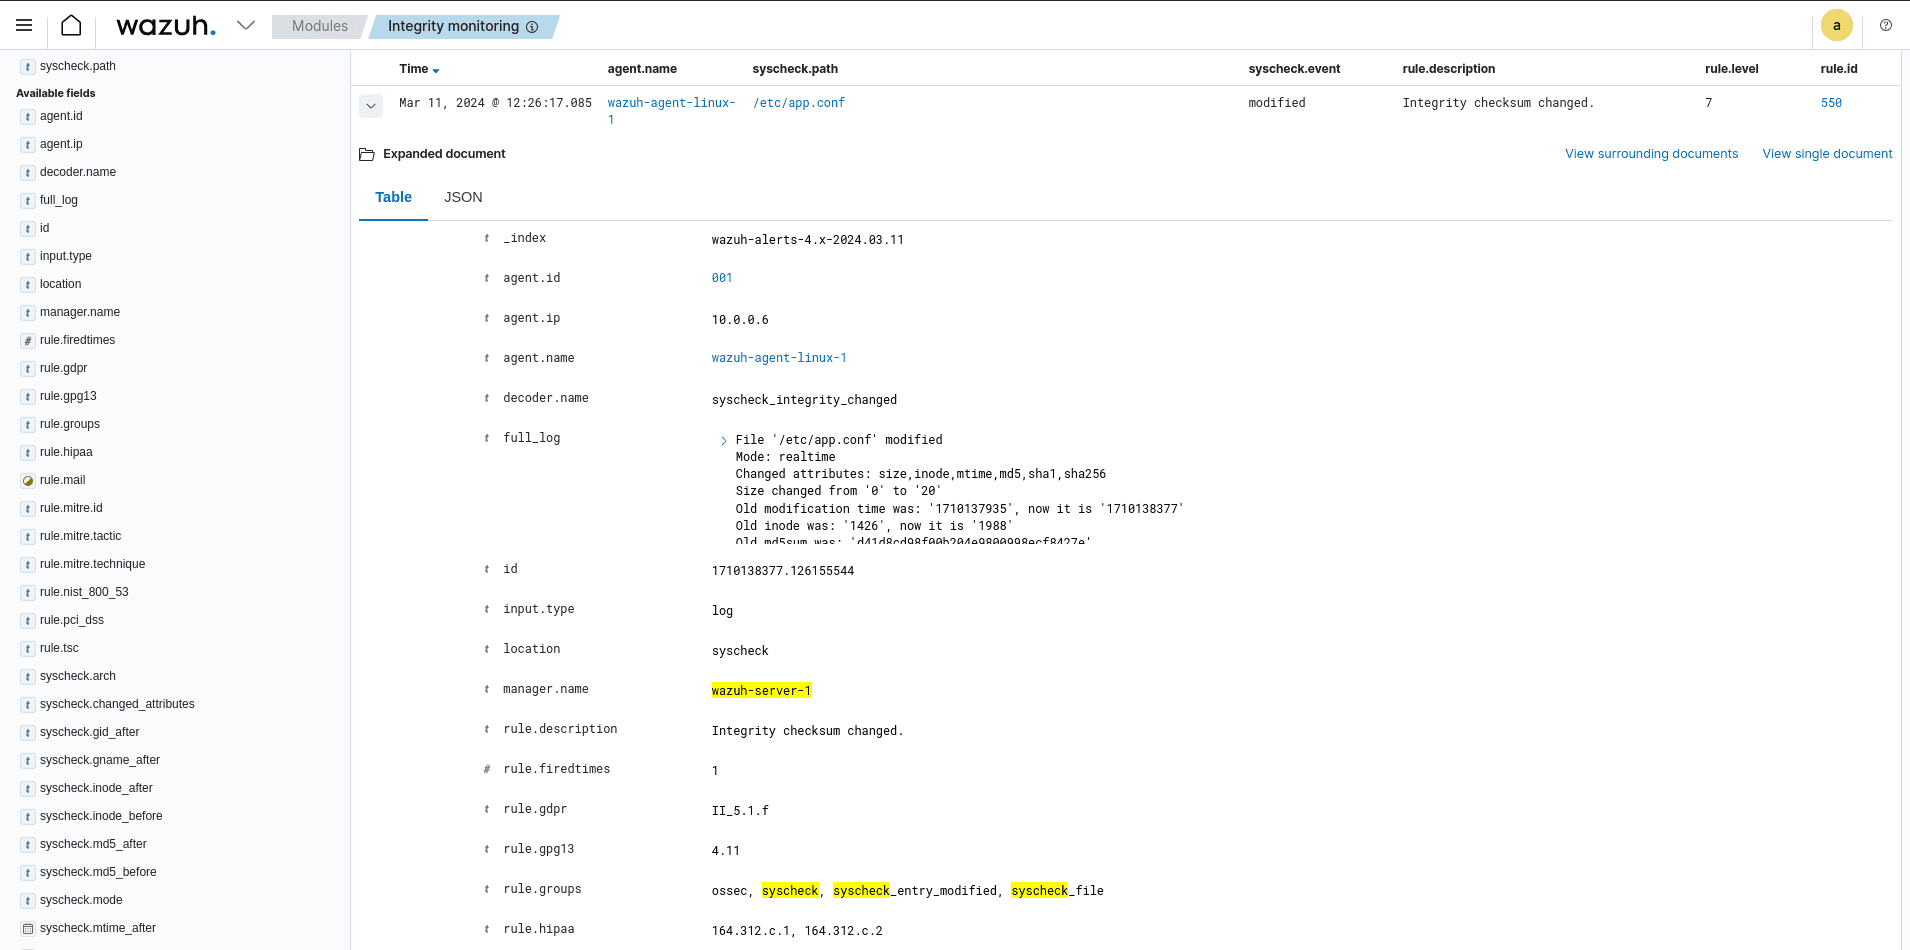
\includegraphics[width=0.75\textwidth]{images/fim/fim-8.png}
              \caption{Alert Details for Change in \texttt{/etc/app.conf} File}
              \label{fig:fim-8}
          \end{figure}

\end{itemize}
